\section{Longstaff \& Schwartz pricing}
Another approach to American option pricing is manifest in the Least
Squares Monte Carlo algorithm, often shortened to LSM. Here Monte
Carlo simulation is used to generate a corpus of possible price
developments of the underlying asset, and the option price is then
calculated by successively applying linear regression at each time
step from expiration to initiation time.

% In a historical context, Monte Carlo methods is relatively new
% approach to option pricing. Lattice methods where introduced in 1973,
% but only since 

\begin{algorithm}
  \begin{algorithmic}
    \Function{LSM}{$T$, $M$, $N$, $S_0$, $K$, $r$}
    \State $\Delta t \gets \frac{T}{M}$
    \State $S \gets$ \Call{GeneratePricePaths}{...} \Comment $S$ is a $N \times (M+1)$ matrix of $N$ paths
    \State $C_0 \gets $ \textbf{parmap} $(\lambda s.\ max(K-s, 0)$ $S_N$ \Comment Initialize cash flow matrix
    \For{$t \gets M-1$ \textbf{to} $1$}
    \State{filter away paths not in the money etc. etc.}
    \State $f_t \gets$ \Call{LeastSquares}{...} \Comment Find regression function $f_t$
    \State estimated time values $\gets$ \textbf{parmap} $f_i$ $S_t$
    \EndFor
    \EndFunction
  \end{algorithmic}
  
  \caption{Least Squares Monte Carlo algorithm}
  \label{alg:lsm-algorithm}
\end{algorithm}

Algorithm \ref{alg:lsm-algorithm} presents the LSM algorithm. We have
left out how to generate price paths and perform least squares
regression, these will be treated in more detail in the subsequent
sections.

\subsection{Path generation}
A standard approach to constructing the corpus of price paths is by
sampling paths of geometric Brownian motion.

This can be done by iterative application of the following equation:
$$S_{t+\Delta t}=S_te^{\Delta t(r-\sigma^2/2) + \sigma v\sqrt{\Delta t}}$$ where 
$v$ is a real number drawn from $\mathcal{N}(0,1)$, $\Delta t$ is the
size of the time period, and $\sigma$ is the volatility. Volatility is
the standard deviation of the option value over time and corresponds
to $u$ and $d$ in the binomial method. The right-hand side consists of
two parts where the first exponent corresponds to the deterministic
evolution of the price by the riskless interest rate, and the second
part corresponds to the variation introduced from the Brownian
motion. A derivation of the equation can be found in the book
\emph{Monte-Carlo Methods in Financial Engineering} by Paul Glasserman
\cite[Section 3.2]{glasserman2003monte}.

\begin{algorithm}
  \begin{algorithmic}
    \Function{GeneratePricePaths}{$N$, $M$, $s_0$, $\sigma$, $\Delta t$, $r$}
    \State $S_0 \gets$ Initialize vector with $N$ repetitions of $s_0$
    \For{$i \gets 0$ \textbf{to} $M-1$}
      \State $V \gets$ Generate $N$ normally distributed random numbers
      \State $D \gets$ \textbf{parmap} $(\lambda v.\ e^{\Delta t(r-\sigma^2/2) + \sigma v\sqrt{\Delta t}})$ $V$
      \State $S_{i+1} \gets$ \textbf{parallelZipWith} $(+)$ $S_{i}$ $D$
    \EndFor
    \State \Return S
    \EndFunction
  \end{algorithmic}
  \caption{Brownian motion path generation}
  \label{alg:lsm-pathgeneration}
\end{algorithm}

\todo{perhaps introduce Brownian Bridge alternative}

As long as we can generate independent random numbers in parallel this
generation can also be parallelized, as each path can be generated
independently.

\subsection{Random number generation}
A necessity for all applications of Monte Carlo methods is a source of
good random numbers. We cannot computationally generate ``true'' random
numbers, as they will always follow our chosen algorithm, but through
the use of \emph{pseudo-random number generators} (PRNGs) we can
generate sequences of numbers with approximately the same properties
as a completely random sequence. Such algorithms are widely used in both
Monte Carlo simulation and cryptography, but the choice of algorithm
depends on the application area as different PRNGs displays different
statistical properties.

An alternative scheme is that of \emph{quasi-random number generators}
(QRNGs). Algorithms in this category aims for sequences with low
discrepancy, which is a measure of spacing in the sequence. If we are
to generate a sequence over some interval $[a,b]$, discrepancy would
be high if there were subintervals $[c,d]$ with proportionally few
samples compared to other intervals. Low discrepancy thus guarantees
that proportionally equal amounts of samples are made in all
subintervals. We thus avoid seing gaps with few or no samples and
regions with high sample density. To illustrate, Figure
\ref{fig:discrepancyplot} shows a graph of a low-discrepancy sequence
compared with sequence of uniformly generated numbers from a PRNG.

\begin{figure}
	\centering
	\subbottom[]{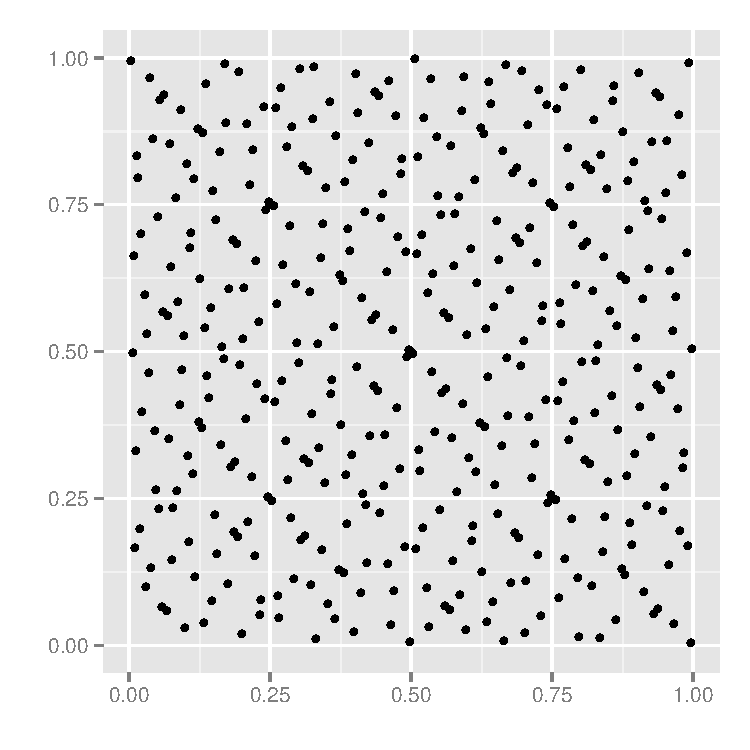
\includegraphics[width=0.45\textwidth]{graphics/2D-sobol-sequence.pdf}\hspace{0.55cm}\label{fig:2d-sobol-sequence}}
	\subbottom[]{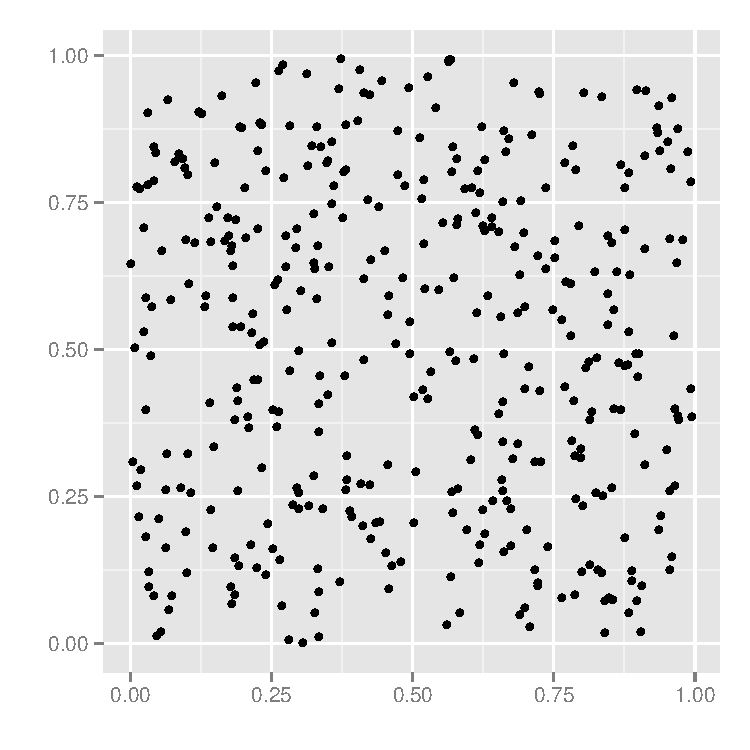
\includegraphics[width=0.45\textwidth]{graphics/2D-mersenne-sequence.pdf}\hspace{0.55cm}}

  \caption{\textbf{(a)} A 2D sequence of low-discrepancy numbers
    generated using the Sobol generator \textbf{(b)} A uniform 2D
    sequence of pseudorandom numbers generated with Mersenne twister
    PRNG}
\label{fig:discrepancyplot}
\end{figure}

QRNGs does not assure any other properties of random sequences and
does indeed follow rather visible patterns (see Figure
\ref{fig:2d-sobol-sequence}). It is not the aim to get close to
statistically random numbers, instead QRNG provides numbers suitable
for numerical integration, optimization and simulation. QRNGs have
several times been shown useful in financial Monte Carlo simulations
\cite{chaudhary2005american, couffignals2010quasi,
  dfine2009americanbasket} \todo{perhaps mention the differences
  between their methods} and a survey paper shows QRNGs beating PRNGs
when it comes to option pricing \cite{acworth1998comparison}. The
survey is a bit old, so newer PRNGs might perform differently.

\todo{see also
  \url{http://en.wikipedia.org/wiki/Quasi-Monte_Carlo_methods_in_finance}}

We will look closer at one particular low-discrepancy generator,
namely the Sobol sequence generator, by the Russian mathematician
I.M. Sobol \cite{sobol1967}. 

\todo{why we choose Sobol over other QRNGs, see above survey, argue
  that we selected it based on its usage in the LexiFi code}

\subsection{Sobol generator}
We will not discuss why the numbers generated by the Sobol generator
maintain low discrepancy, but only focus on the algorithmic aspect of
computing the numbers.

Given a sequence of so called \emph{direction numbers}, $v_1, v_2,
\ldots$, the computation of Sobol-sequences is pretty straight forward:
$$x_i = b_1v_1 \oplus b_2v_2 \oplus \ldots$$
where $\ldots b_3b_2b_1$ is the binary representation of $i$. This
simple algorithm is presented in Figure \ref{alg:sobol-inductive},
where \textsc{ToBitVector} converts an integer $i$ to its binary
representation as an array of integers. As each iteration is
independent, we can parallelise this by mapping
\textsc{SobolInductive} over the indices.

\begin{algorithm}
  \begin{algorithmic}
    \Function{SobolInductive}{$v$,$i$}
    \State \Return \textbf{fold} $\oplus$ 0 (\textbf{zipWith} ($\times$) $v$ (\textsc{ToBitVector} $i$))
    \EndFunction
  \end{algorithmic}
  \caption{Generate element $i$ of the Sobol sequence using vector
    $v$ as direction numbers.}
  \label{alg:sobol-inductive}
\end{algorithm}

% \begin{algorithm}
%   \begin{algorithmic}
%     \Function{SobolInductive}{$v$,$n$}
%     \ParFor{$i \gets 0$ to $n-1$}
%     \State $A[i] \gets$ \textbf{fold} $\oplus$ 0 (\textbf{zipWith} ($\times$) (\textsc{ToBitVector} i) $v$)
%     \EndParFor
%     \EndFunction
%   \end{algorithmic}
%   \caption{Inductive Sobol generator.}
%   \label{alg:sobol-inductive}
% \end{algorithm}

If one seeks for a sequential algorithm, we can improve by using the
Gray code binary representation of the index instead of the ordinary,
whereby a recursive definition of Sobol sequences can be made
\todo{ref}. It has been shown that
$$x_{i+1} = x_n \oplus v_c$$
where $c = \mathit{lsb}(n)$ is the index of the least set bit in
$n$. A sequential algorithm using this strategy is presented in Figure
\ref{alg:sobol-recursive}.

\begin{algorithm}
  \begin{algorithmic}
    \Function{SobolRecursive}{$v$,$A$,$i$,$n$}
    \State $A[i] \gets$ \textsc{SobolInductive} (\textsc{GrayCode} $i$)
    \State $j \gets i + 1$
    \While{$j < i + n$ \textbf{and} $j < length[A]$}
    \State $c \gets \mathrm{lsb}(j)$
    \State $A[j] \gets A[j-1] \oplus v_c$
    \State $j \gets j + 1$
    \EndWhile
    \EndFunction
  \end{algorithmic}
  \caption{Generate elements $i$ through $i+n-1$ of the Sobol
    sequence and store results at the appropriate indices of $A$}
  \label{alg:sobol-recursive}
\end{algorithm}

You will not obtain the same sequence using this approach though, but
it has been shown \todo{cite} that Gray code based sequences also
displays the property of low discrepancy, as it is merely a scrambling
(reordering) of prefixes of the original Sobol sequence. As conversion
to Gray code representation is done through single shift and an
exclusive-or operation, this makes for a cheap sequential algorithm.

The two approaches can be combined to achieve an alternative parallel
implementation. The sequence that needs to be generated is divided in
chunks onto each processing element, the inductive algorithm is used
to initialize each of the chunks and the recursive algorithm is then
used to fill out the space. The algorithm is shown in Figure
\ref{alg:sobol-parallel-1}

\begin{algorithm}
  \todo{remember to normalise to $(0,1]$}
  \begin{algorithmic}
    \Function{SobolParRecurse}{$v$,$n$}
    \State $m \gets$ number of processor cores
    \State $r \gets \lfloor n/m \rfloor$
    \ParFor{$p \gets 0$ to $m-1$}
    \State $start \gets p\cdot r$
    \State \textsc{SobolRecursive}($v$,$A$,$start$,$\min(r,n-start)$)
    \EndParFor
    \EndFunction
  \end{algorithmic}
  \caption{Parallel Sobol sequence generator.}
  \label{alg:sobol-parallel-1}
\end{algorithm}

The problem with this algorithm is that its memory behavior is not
suitable for GPUs. Programs that does not coalesce memory accesses,
such that all cores act on the same block simultaneously, incurs a big
performance penalty. With this algorithm, each thread will write very
dispersed, as each thread will fill out each its own region of the
array A.

Luckily, an alternative strategy has been shown by Thomas Bradley et
al. \cite{bradley2010parallelisation} \todo{It seems that this might
  actually be a chapter from the book ``GPU Computing Gems Emerald
  Edition'', change citation accordingly?}.

\begin{algorithm}
  \todo{remember to normalise to $(0,1]$}
  \todo{define that $m$ is per SM}
  \begin{algorithmic}
    \Function{SobolSkipping}{$v$,$n$}
    \State $m \gets$ number of processor cores
    \State $r \gets \lfloor n/m \rfloor$
    \ParFor{$p \gets 0$ \textbf{to} $m-1$}
    \State $A[p] \gets$ \textsc{SobolInductive} (\textsc{GrayCode} $p$)
    \State $i \gets p + m$
    \While{$i < n$}
    \State $A[i] \gets A[i - 1] \oplus \ldots$
    \State $i <- i + m$
    \EndWhile
    \EndParFor
    \EndFunction
  \end{algorithmic}
  \caption{Parallel Sobol sequence generator.}
  \label{alg:sobol-parallel-1}
\end{algorithm}


\subsection{Sampling the standard normal distribution}
The Sobol sequence generator as well as most other PRNG's and QRNG's
draws samples uniformly from the interval $(0,1]$ ($0$ is not
included, as we often want to avoid negative samples). In our
application we need samples from the standard normal distribution,
$\mathcal{N}(0,1)$, and thus a transformation is necessary. We have
not looked closely at this particular aspect, and thus have just
settled on using the pretty simple Box-Muller transformation. With
Box-Muller a pair of independent random variates $u,v$ drawn uniformly
from $(0,]$ can be transformed into two values $x,y$ of the standard normal
distribution by:

\begin{equation*}
  x =\sqrt{-2 \ln u} \cos(2 \pi v) \quad\quad
  y = \sqrt{-2 \ln u} \sin(2 \pi v)
\end{equation*}

It is thus easy to parallelise, as there are only dependency between
every two samples, but the $\cos$ and $\sin$ operations are quite
expensive. \todo{maybe a footnote on using CUDA's
  \emph{sincospi}-function that implements $\mathrm{sincospi}(x) = \sin(\pi \cdot x)$ and
  $\cos(\pi \cdot x)$}

\subsection{Least Squares solvers}
\todo{LU, QR and Cholesky decomposition}

%%% Local Variables:
%%% mode: latex
%%% TeX-master: "../master"
%%% End:
